\documentclass[12pt]{article}
\usepackage{graphicx}
\usepackage{geometry}
\usepackage{amsmath}
\usepackage{hyperref}
\usepackage{listings}
\usepackage{color}
\usepackage{float}
\geometry{margin=1in}
\setlength{\parskip}{1em}

\title{\textbf{Experiment 2: Spam or Ham Classification using Na\"ive Bayes, KNN, and SVM with Hyperparameter Optimization}}
\author{Machine Learning Lab Report}
\date{Academic Year 2025--2026}

\definecolor{codegray}{rgb}{0.5,0.5,0.5}
\definecolor{codepurple}{rgb}{0.58,0,0.82}
\definecolor{backcolour}{rgb}{0.95,0.95,0.92}
\lstdefinestyle{mystyle}{
    backgroundcolor=\color{backcolour},
    commentstyle=\color{codegray},
    keywordstyle=\color{blue},
    numberstyle=\tiny\color{codegray},
    stringstyle=\color{codepurple},
    basicstyle=\ttfamily\footnotesize,
    breaklines=true,
    captionpos=b,
    keepspaces=true,
    numbers=left,
    numbersep=5pt,
    showspaces=false,
    showstringspaces=false,
    showtabs=false,
    tabsize=2
}
\lstset{style=mystyle}

\begin{document}
\maketitle

\section*{Aim}
To classify emails as spam or ham using Na\"ive Bayes, K-Nearest Neighbors (KNN), and Support Vector Machine (SVM), and to evaluate their performance using standard classification metrics, K-Fold cross-validation, and hyperparameter optimization via GridSearchCV.

\section*{Libraries Used}
\begin{itemize}
\item pandas
\item numpy
\item matplotlib
\item seaborn
\item scikit-learn
\end{itemize}

\section*{Objective}
\begin{itemize}
\item Load and preprocess the dataset
\item Perform exploratory data analysis (EDA)
\item Train classifiers: Na\"ive Bayes, KNN, and SVM
\item Optimize KNN and SVM hyperparameters using GridSearchCV
\item Evaluate using accuracy, precision, recall, F1-score, confusion matrix, and ROC curve
\item Compare performance using 5-fold cross-validation
\end{itemize}

\section*{Code Snippets}
\textbf{1. Data Loading and Preprocessing:}
\begin{lstlisting}[language=Python]
df = pd.read_csv("spambase_csv.csv")
df.fillna(df.mean(), inplace=True)
X_raw = df.drop(columns=['class'])
y = df['class']
\end{lstlisting}

\textbf{2. Train-Test Split and Scaling:}
\begin{lstlisting}[language=Python]
from sklearn.model_selection import train_test_split
from sklearn.preprocessing import StandardScaler

X_train_raw, X_test_raw, y_train_raw, y_test_raw = train_test_split(
    X_raw, y, test_size=0.2, random_state=42
)

scaler = StandardScaler()
X_scaled = scaler.fit_transform(X_raw)
X_train_scaled, X_test_scaled, y_train_scaled, y_test_scaled = train_test_split(
    X_scaled, y, test_size=0.2, random_state=42
)
\end{lstlisting}

\textbf{3. Evaluation Function:}
\begin{lstlisting}[language=Python]
from sklearn.metrics import accuracy_score, precision_score, recall_score, f1_score, confusion_matrix, roc_curve, auc

def evaluate(name, model, X_test, y_test):
    y_pred = model.predict(X_test)
    acc = accuracy_score(y_test, y_pred)
    prec = precision_score(y_test, y_pred)
    rec = recall_score(y_test, y_pred)
    f1 = f1_score(y_test, y_pred)
    print(f"{name} -- Accuracy: {acc:.2f}, Precision: {prec:.2f}, Recall: {rec:.2f}, F1 Score: {f1:.2f}")
\end{lstlisting}

\textbf{4. Training Gaussian Na\"ive Bayes:}
\begin{lstlisting}[language=Python]
from sklearn.naive_bayes import GaussianNB
model = GaussianNB()
model.fit(X_train_raw, y_train_raw)
evaluate("GaussianNB", model, X_test_raw, y_test_raw)
\end{lstlisting}

\textbf{5. KNN with GridSearchCV for Optimal k:}
\begin{lstlisting}[language=Python]
from sklearn.model_selection import GridSearchCV
from sklearn.neighbors import KNeighborsClassifier

param_grid = {'n_neighbors': [1, 3, 5, 7]}
knn = KNeighborsClassifier()
knn_grid = GridSearchCV(knn, param_grid, cv=5, scoring='accuracy', n_jobs=-1)
knn_grid.fit(X_train_scaled, y_train_scaled)
best_k = knn_grid.best_params_['n_neighbors']

# Evaluate best K
best_knn = knn_grid.best_estimator_
evaluate(f"KNN (Best k={best_k})", best_knn, X_test_scaled, y_test_scaled)
\end{lstlisting}

\textbf{6. KNN KDTree vs BallTree:}
\begin{lstlisting}[language=Python]
knn_kd = KNeighborsClassifier(n_neighbors=best_k, algorithm='kd_tree')
knn_kd.fit(X_train_scaled, y_train_scaled)
evaluate(f"KNN - KDTree (k={best_k})", knn_kd, X_test_scaled, y_test_scaled)

knn_bt = KNeighborsClassifier(n_neighbors=best_k, algorithm='ball_tree')
knn_bt.fit(X_train_scaled, y_train_scaled)
evaluate(f"KNN - BallTree (k={best_k})", knn_bt, X_test_scaled, y_test_scaled)
\end{lstlisting}

\textbf{7. SVM with GridSearchCV for Different Kernels:}
\begin{lstlisting}[language=Python]
from sklearn.svm import SVC

# Linear
param_grid_linear = {'C':[0.1,1,10]}
grid_linear = GridSearchCV(SVC(kernel='linear', probability=True), param_grid_linear, cv=5)
grid_linear.fit(X_train_scaled, y_train_scaled)
evaluate(f"SVM - Linear (C={grid_linear.best_params_['C']})", grid_linear.best_estimator_, X_test_scaled, y_test_scaled)

# Polynomial
param_grid_poly = {'C':[0.1,1,10], 'degree':[2,3,4], 'gamma':['scale','auto']}
grid_poly = GridSearchCV(SVC(kernel='poly', probability=True), param_grid_poly, cv=5)
grid_poly.fit(X_train_scaled, y_train_scaled)
best_poly = grid_poly.best_estimator_
evaluate(f"SVM - Polynomial {grid_poly.best_params_}", best_poly, X_test_scaled, y_test_scaled)

# RBF
param_grid_rbf = {'C':[0.1,1,10], 'gamma':['scale','auto']}
grid_rbf = GridSearchCV(SVC(kernel='rbf', probability=True), param_grid_rbf, cv=5)
grid_rbf.fit(X_train_scaled, y_train_scaled)
best_rbf = grid_rbf.best_estimator_
evaluate(f"SVM - RBF {grid_rbf.best_params_}", best_rbf, X_test_scaled, y_test_scaled)

# Sigmoid
param_grid_sig = {'C':[0.1,1,10], 'gamma':['scale','auto']}
grid_sig = GridSearchCV(SVC(kernel='sigmoid', probability=True), param_grid_sig, cv=5)
grid_sig.fit(X_train_scaled, y_train_scaled)
best_sig = grid_sig.best_estimator_
evaluate(f"SVM - Sigmoid {grid_sig.best_params_}", best_sig, X_test_scaled, y_test_scaled)
\end{lstlisting}

\section*{Results and Comparisons}

\subsection*{Table 1: Naïve Bayes Performance}
\begin{tabular}{|l|c|c|c|c|}
\hline
\textbf{Model} & \textbf{Accuracy} & \textbf{Precision} & \textbf{Recall} & \textbf{F1 Score} \\
\hline
GaussianNB & 0.820847 & 0.719298 & 0.946154 & 0.817276 \\
MultinomialNB & 0.786102 & 0.764384 & 0.715385 & 0.739073 \\
BernoulliNB & 0.880565 & 0.906977 & 0.800000 & 0.850136 \\
\hline
\end{tabular}

\subsection*{Table 2: KNN (GridSearchCV) Performance}
\begin{tabular}{|l|c|c|c|c|}
\hline
\textbf{Model} & \textbf{Accuracy} & \textbf{Precision} & \textbf{Recall} & \textbf{F1 Score} \\
\hline
Best KNN (k=7) & 0.895765 & 0.910615 & 0.835897 & 0.871658 \\
1 & 0.895765 & 0.876923 & 0.876923 & 0.876923 \\
3 & 0.893594 & 0.888298 & 0.856140 & 0.872063 \\
5 & 0.895765 & 0.901639 & 0.846154 & 0.873016 \\
\hline
\end{tabular}

\subsection*{Table 3: KNN KDTree vs BallTree Performance}
\begin{tabular}{|l|c|c|}
\hline
\textbf{Metric} & \textbf{KDTree} & \textbf{BallTree} \\
\hline
Accuracy & 0.895765 & 0.895765 \\
Precision & 0.910615 & 0.910615 \\
Recall & 0.835897 & 0.835897 \\
F1 Score & 0.871658 & 0.871658 \\
Training Time (s) & 0.895523 & 0.908345 \\
\hline
\end{tabular}

\subsection*{Table 4: SVM (GridSearchCV) Performance}
\begin{tabular}{|l|l|c|c|c|c|c|}
\hline
\textbf{Kernel} & \textbf{Best Hyperparameters} & \textbf{Accuracy} & \textbf{Precision} & \textbf{Recall} & \textbf{F1 Score} & \textbf{CV Score} \\
\hline
Linear & \{C=1, kernel=linear\} & 0.925081 & 0.934959 & 0.884615 & 0.909091 & 0.928804 \\
Polynomial & \{C=10, degree=2, gamma=scale\} & 0.918567 & 0.941176 & 0.861538 & 0.899598 & 0.911685 \\
RBF & \{C=1, gamma=scale\} & 0.934853 & 0.950820 & 0.892308 & 0.920635 & 0.931250 \\
Sigmoid & \{C=0.1, gamma=scale\} & 0.891422 & 0.921512 & 0.812821 & 0.863760 & 0.890217 \\
\hline
\end{tabular}

\subsection*{Table 5: K-Fold CV Accuracies (K=5)}
\begin{tabular}{|l|c|c|c|c|c|c|}
\hline
\textbf{Fold} & \textbf{GaussianNB} & \textbf{Best KNN} & \textbf{Linear SVM} & \textbf{Poly SVM} & \textbf{RBF SVM} & \textbf{Sigmoid SVM} \\
\hline
1 & 0.820847 & 0.895765 & 0.925081 & 0.918567 & 0.934853 & 0.891422 \\
2 & 0.817391 & 0.913043 & 0.928261 & 0.925000 & 0.933696 & 0.895652 \\
3 & 0.801087 & 0.913043 & 0.916304 & 0.919565 & 0.922826 & 0.894565 \\
4 & 0.820652 & 0.900000 & 0.936957 & 0.919565 & 0.935870 & 0.902174 \\
5 & 0.835870 & 0.911957 & 0.930435 & 0.915217 & 0.930435 & 0.891304 \\
\hline
\textbf{Average} & 0.819169 & 0.906762 & 0.927408 & 0.919583 & 0.931536 & 0.895024 \\
\hline
\end{tabular}

\section*{ROC Curves and Confusion Matrices}
Each model’s ROC curve and confusion matrix are shown below:

% Naive Bayes
\begin{figure}[H]
\centering
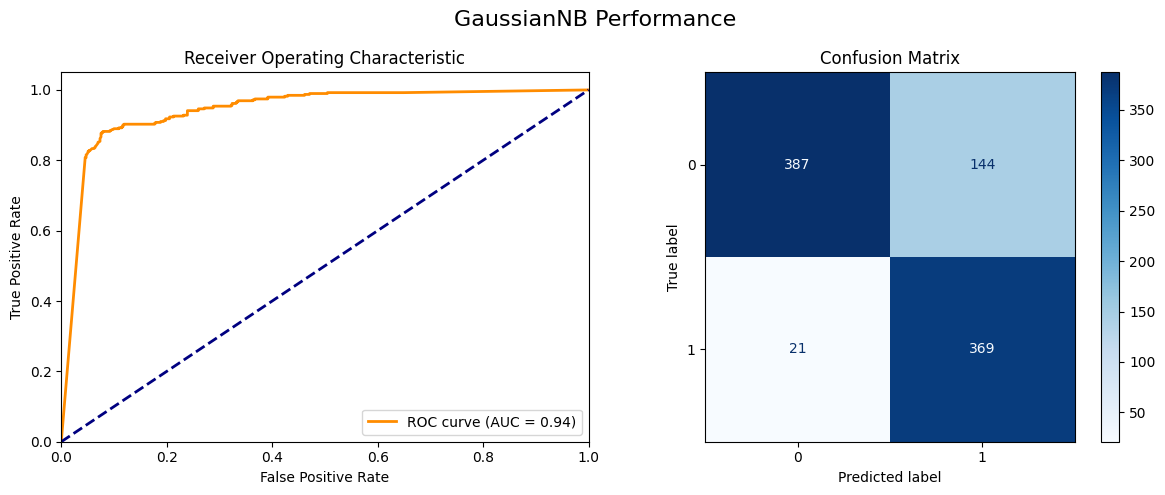
\includegraphics[width=1\textwidth]{images/naivebayes1.png}
\caption{Gaussian Na\"ive Bayes Results}
\end{figure}

\begin{figure}[H]
\centering
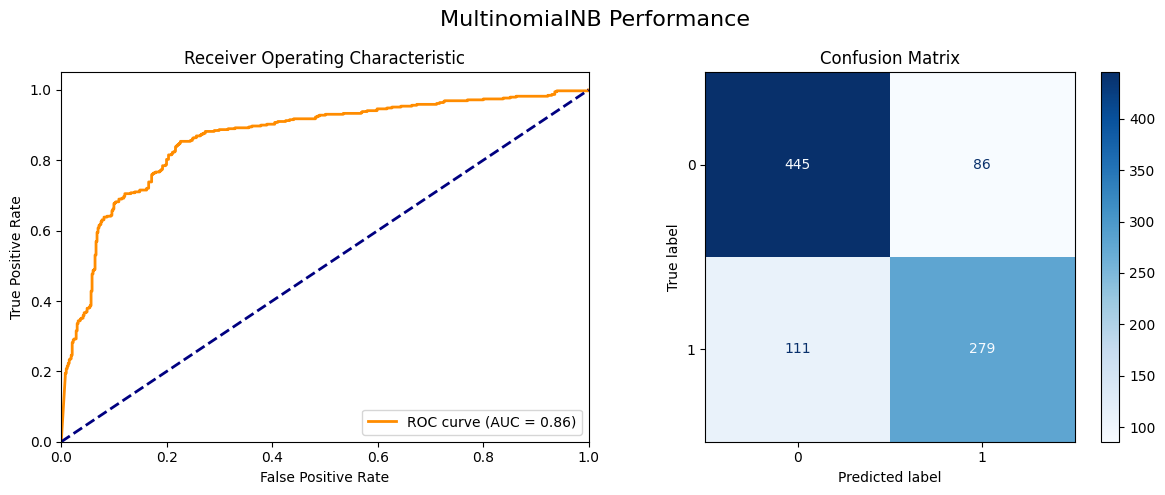
\includegraphics[width=1\textwidth]{images/naivebayes2.png}
\caption{Multinomial Na\"ive Bayes Results}
\end{figure}

\begin{figure}[H]
\centering
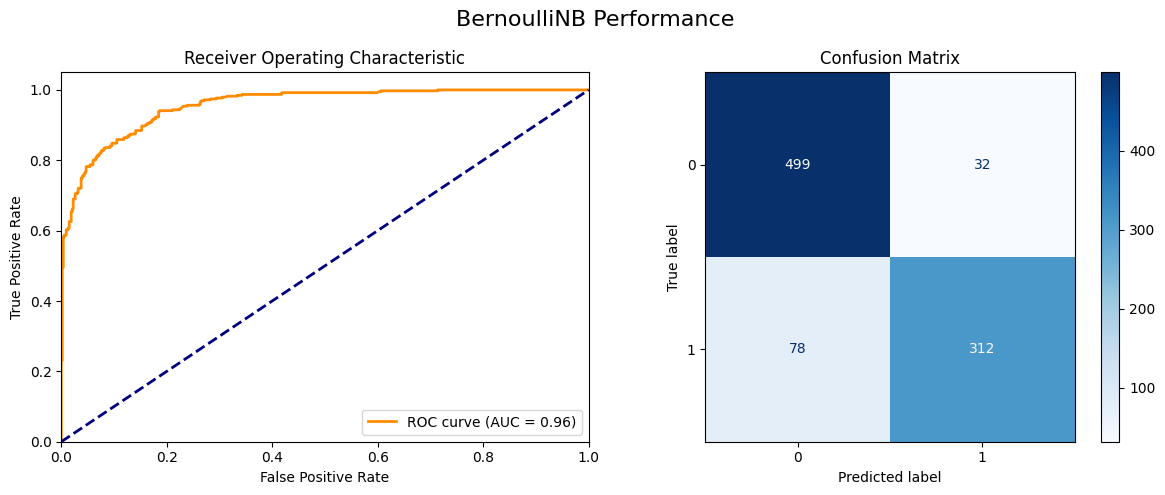
\includegraphics[width=1\textwidth]{images/naivebayes3.png}
\caption{Bernoulli Na\"ive Bayes Results}
\end{figure}

% KNN K=1
\begin{figure}[H]
\centering
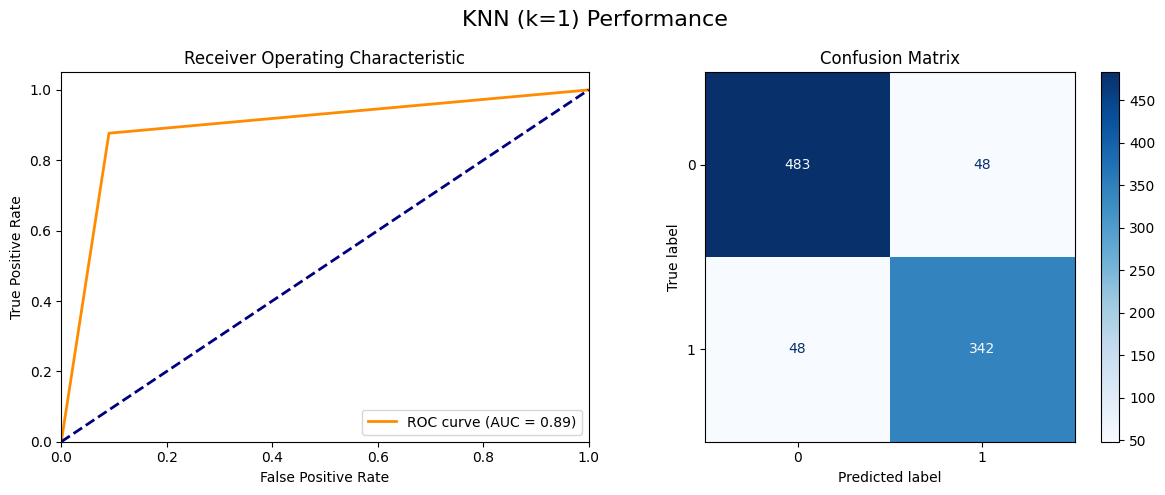
\includegraphics[width=1\textwidth]{images/knn1.png}
\caption{K-Nearest Neighbors (k=1) Results}
\end{figure}
% KNN K=3
\begin{figure}[H]
\centering
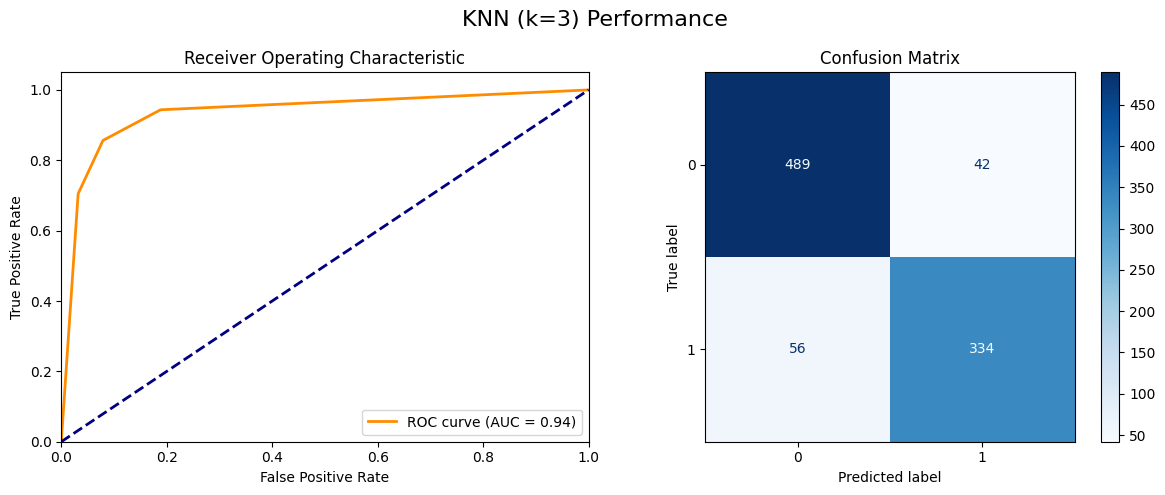
\includegraphics[width=1\textwidth]{images/knn2.png}
\caption{K-Nearest Neighbors (k=3) Results}
\end{figure}

% KNN K=5
\begin{figure}[H]
\centering
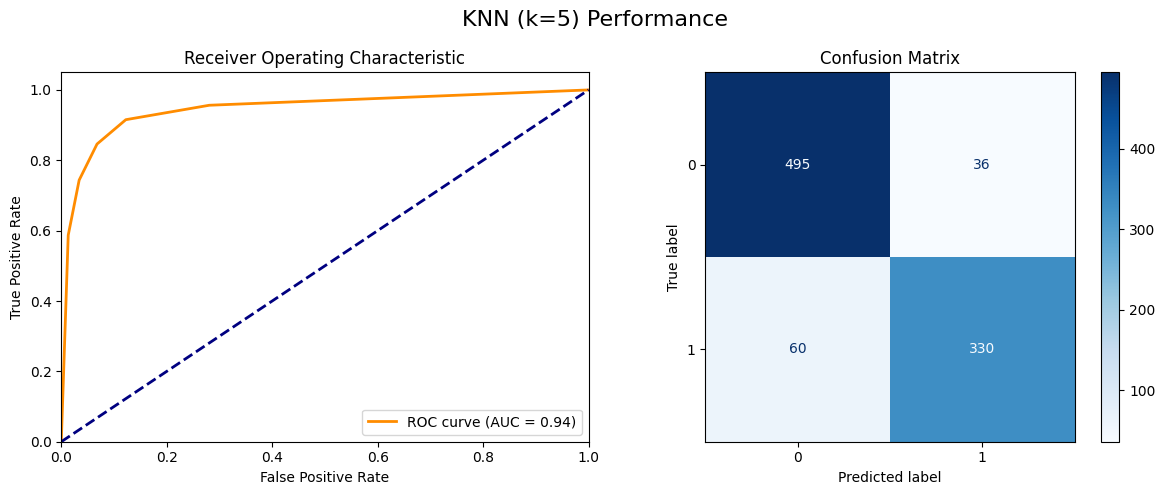
\includegraphics[width=1\textwidth]{images/knn3.png}
\caption{K-Nearest Neighbors (k=5) Results}
\end{figure}

% KNN K=7
\begin{figure}[H]
\centering
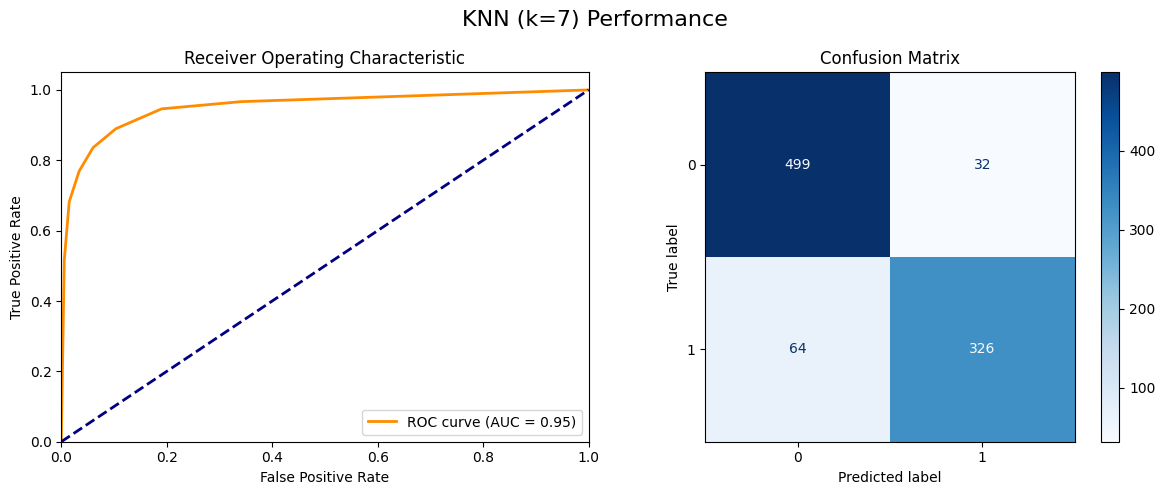
\includegraphics[width=1\textwidth]{images/knn4.png}
\caption{K-Nearest Neighbors (k=7) Results}
\end{figure}

% KNN KD
\begin{figure}[H]
\centering
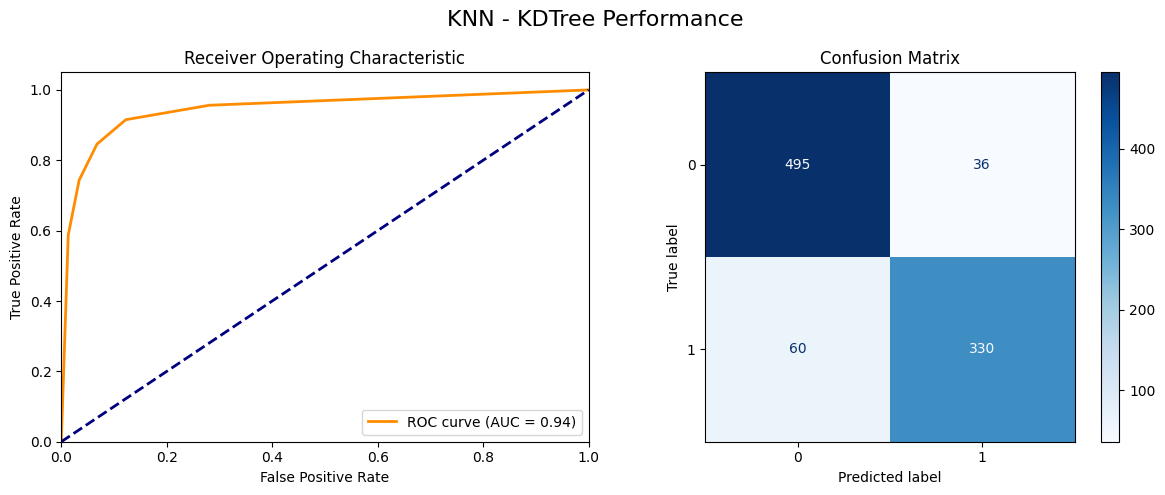
\includegraphics[width=1\textwidth]{images/knn5.png}
\caption{K-Nearest Neighbors (KDTree) Results}
\end{figure}

% KNN ball
\begin{figure}[H]
\centering
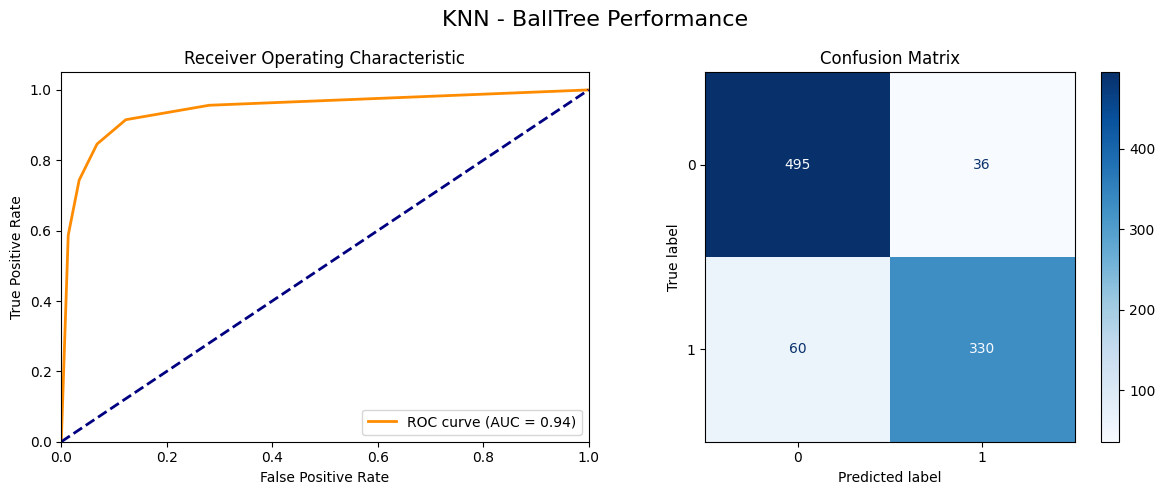
\includegraphics[width=1\textwidth]{images/knn6.png}
\caption{K-Nearest Neighbors (BallTree) Results}
\end{figure}
% SVM
\begin{figure}[H]
\centering
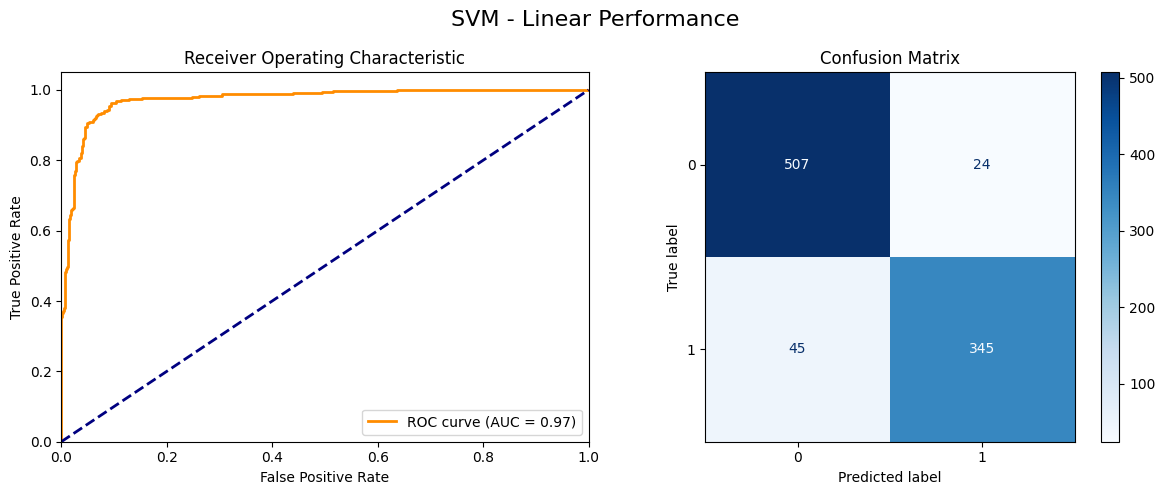
\includegraphics[width=1\textwidth]{images/svm1.png}
\caption{SVM (Linear Kernel) Results}
\end{figure}

\begin{figure}[H]
\centering
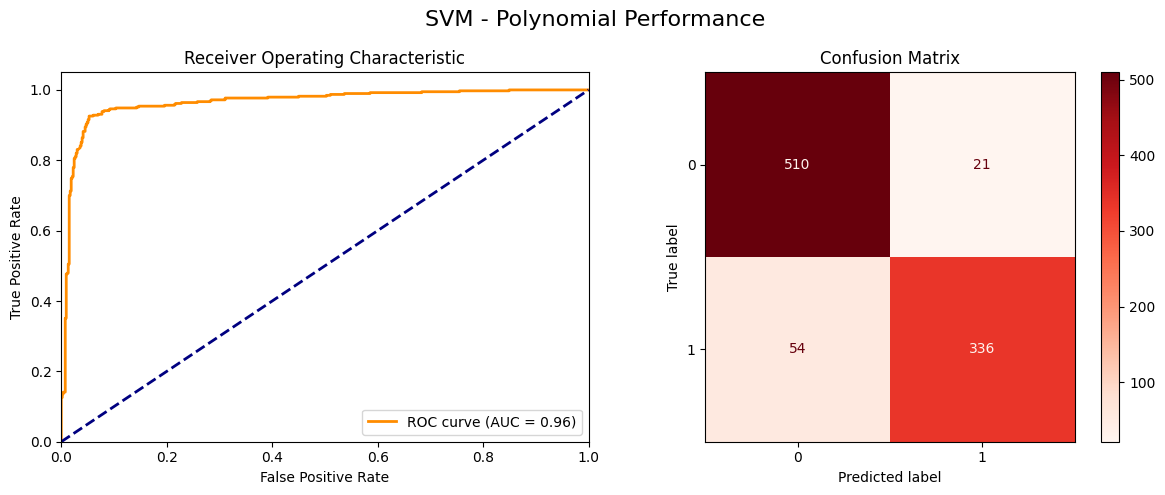
\includegraphics[width=1\textwidth]{images/svm2.png}
\caption{SVM (Polynomial Kernel) Results}
\end{figure}

\begin{figure}[H]
\centering
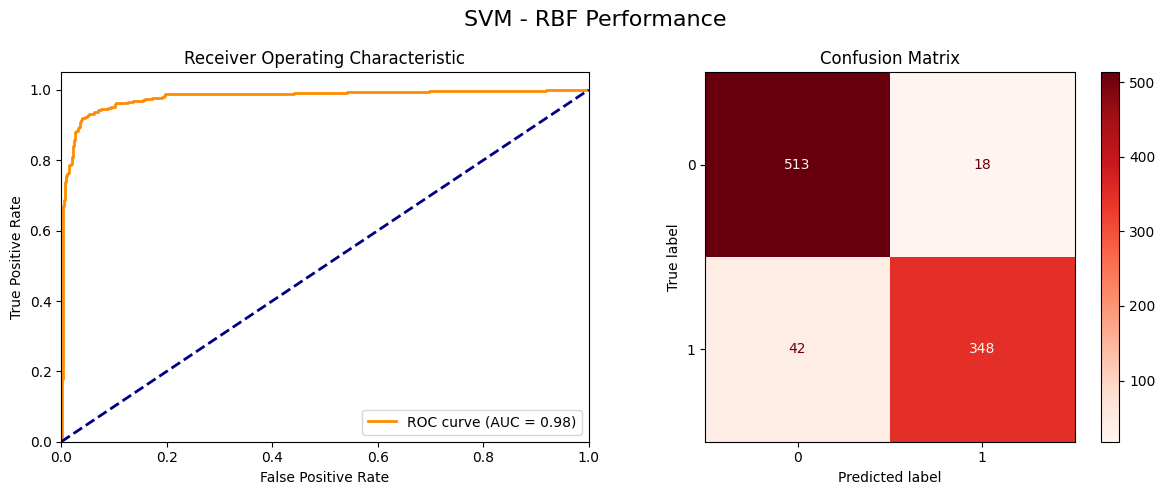
\includegraphics[width=1\textwidth]{images/svm3.png}
\caption{SVM (RBF Kernel) Results}
\end{figure}

\begin{figure}[H]
\centering
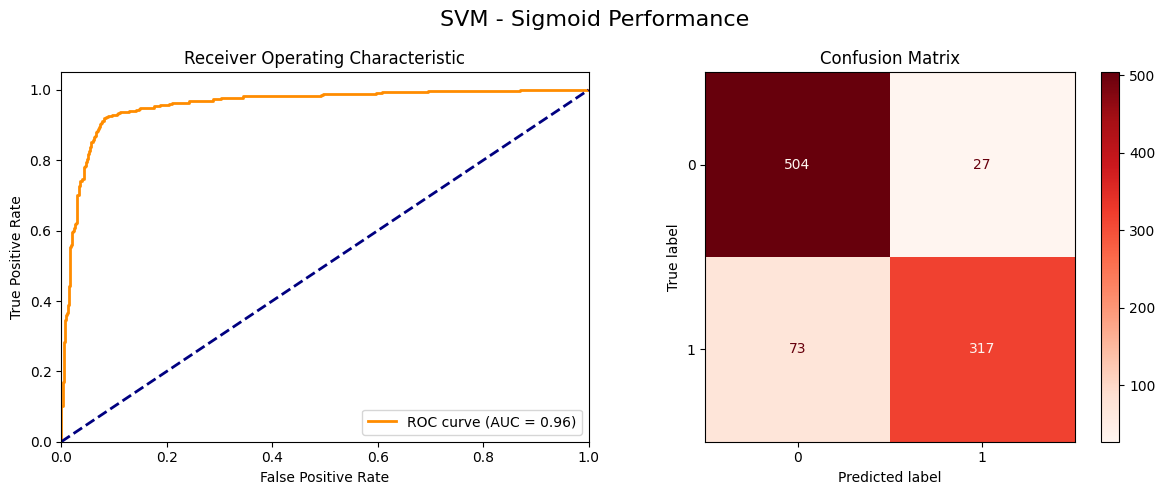
\includegraphics[width=1\textwidth]{images/svm4.png}
\caption{SVM (Sigmoid Kernel) Results}
\end{figure}

\section*{Conclusion}
In this experiment, we implemented and evaluated Na\"ive Bayes, KNN, and SVM classifiers on the Spambase dataset.  
\begin{itemize}
\item \textbf{Na\"ive Bayes:} Fastest, but GaussianNB and BernoulliNB performed better than MultinomialNB.  
\item \textbf{KNN:} Best result at \(k=7\). KDTree and BallTree yielded identical accuracy and F1-scores.  
\item \textbf{SVM:} RBF kernel achieved the highest performance overall with 93.5\% accuracy and F1-score of 0.921.  
\item \textbf{Cross-validation:} SVM (RBF) consistently outperformed others across folds.  
\end{itemize}

Thus, SVM with RBF kernel is the most suitable model for spam classification in this study.
\end{document}